\chapter{Parameter Estimation Process}
\label{ch: Estimation}

Parameter estimation problems can be interpreted as optimization problems, where one must find the optimal values of parameters in order to reduce error between real system and model when the same disturbance is applied to it. the error vector $e$ at any instant $t$ is calculated as the difference between the output vectors $y_{r}$, measured on the real system, and $y$, obtained from the model equations, as presented below.

\begin{equation}
	e(t) = y_{r}(t) - y(t)
	\label{eq: error_vector}
\end{equation}

The $l^{2}$-norm of error vector, denoted by $J$, is applied to evaluate how well the model describes the real system behaviour. The norm is obtained through equation \eqref{eq: J(p)}. It is important to notice that, since $y$ varies with $p$, so does $J$. The constant $\frac{1}{2}$ is only used for further simplification.

\begin{equation}
	J(p) = \frac{1}{2} \int\displaylimits_{0}^{T_{0}}\lVert e(t)\rVert_{2}dt = \frac{1}{2}\int\displaylimits_{0}^{T_{0}}e(t)^{T}\cdot e(t)dt
	\label{eq: J(p)}
\end{equation}

Many methods were developed for solving optimization problems, but two approaches have been largely employed during the last years. The first approach applies metaheuristics to obtain a sufficiently good solution. These methods are used in a variety of fields, ranging from biology to engineering, due to the fact that they are not developed for a specific type of problem.

Metaheuristics employ a stochastic search to find near-optimal solutions inside a given region. However, those methods often take a great amount of time to converge to a solution \cite{Blum2003}. Examples of metaheuristics are Ant Colony Optimization, Differential Evolution, Particle Swarm Optimization and Genetic Algorithm. Applications of this approach in electrical power system cases can be found in \cite{Todorovski2006} and \cite{Yoshida2000}.

The second approach applies analytical methods to find the local optimum solution from equations derived from the problem. Thus, they are problem specific and must be adapted from one case to another. Analytical methods often converge in few iterations, reducing processing time, but they are sensitive to initial conditions. Some examples of analytical methods are Newton's Method, Kalman Filter, Unscented Kalman Filter, etc.

By combining both approaches, the resulting method is expected to reduce the effects of their disadvantages and improving overall convergence. Mean-Variance Mapping Optimization (MVMO) was the metaheuristic chosen for this problem, alongside Trajectory Sensitivity Method (TSM) as analytical method. Both methods will be discussed in the following sections.

\section{Mean-Variance Mapping Optimization Method}

Presented in \cite{Erlich2010}, this metaheuristic based in evolution of populations shares characteristics with other evolutionary algorithms, but differ from them on how to induce mutations on the offspring in order to diversify the population. By considering statistical data of population during mutation process, MVMO introduces a memory factor to it, enhancing search mechanism. Due this factor, MVMO performs better than similar metaheuristics when population size is relatively small \cite{Nakawiro2011}. The terms `gene', `individuals' and `population' refer to `parameter', `parameter vector' and `set of parameter vectors' in MVMO, for the sake of analogy.

Two other relevant concepts largely used on metaheuristics are exploration and exploitation. The first one refers to a broad search carried through the region of interest. On the other hand, exploitation means the search on a small neighbourhood close to the best solutions.

Before starting the parameter search process, a few settings must be done, such as population size, number of offspring, number of genes selected for mutation and selection method. Also, the search region is defined by setting the range within genes can vary. This constrains the parameters values within a feasible region, preventing divergence. The search region is later normalized for all genes, aiding the estimation process. Termination criteria is also set in this step. In this work, both number of generations and error will be used as stop criteria.

After that, a randomly-distributed population is generated, evaluated and sorted. Moreover, the mean and variance of every gene in each population are calculated. These values will later be used on the mutation process. The individual with lower error is selected as parent for a new generated individual. The offspring is then created following three steps common in evolutionary algorithms: gene selection, mutation and crossover. After creation, the offspring is introduced to the population and the worst individual is discarded, as depicted in Figure \ref{fig: MVMOprocess}.

\begin{figure}[h]
	\caption{Exemplification of MVMO process}
	\begin{center}
		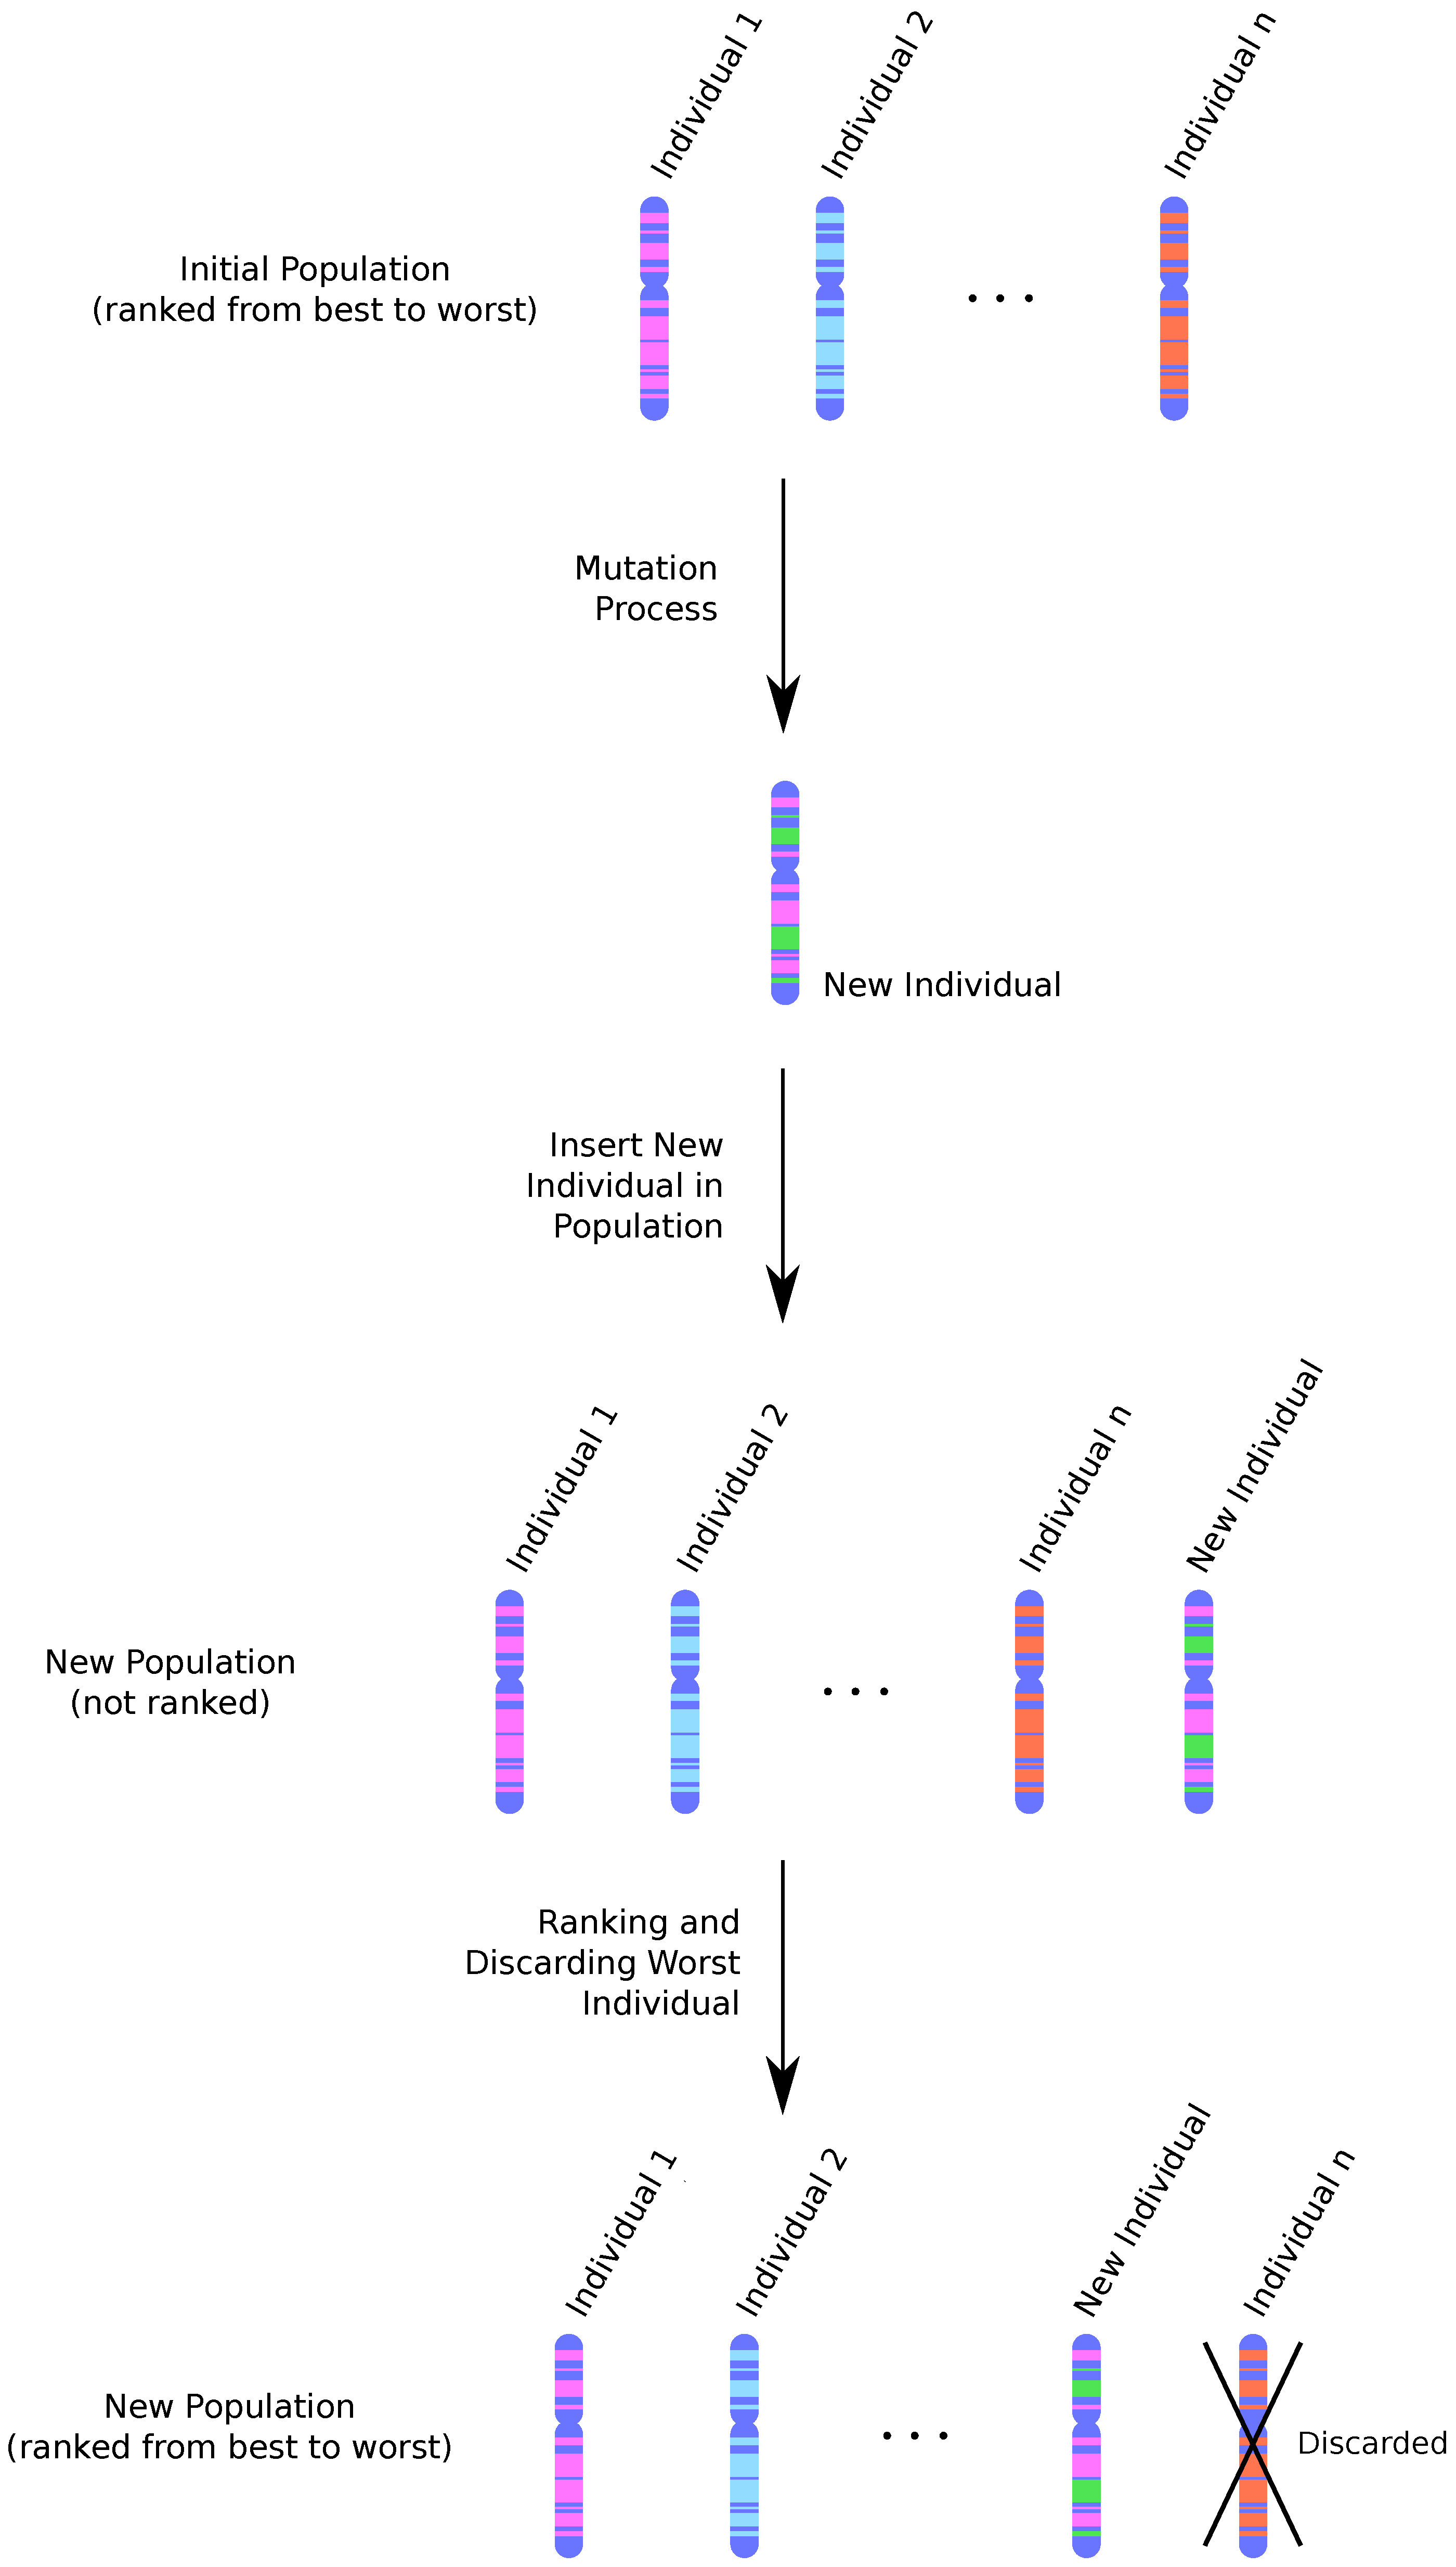
\includegraphics[scale=.2]{Images/MVMO_process2.eps}
	\end{center}
	\label{fig: MVMOprocess}
\end{figure}

\textbf{Gene selection} can be done in many ways and even vary throughout the estimation process, with strategies' efficiency depending on the problem. However, three strategies are commonly used in this step. The first one is comprised of randomly selecting which genes will suffer mutation and which will be directly inherited from the parent. Gene selection can also be done by a moving window approach or even a combination of both strategies, with part of the genes selected at random and other through the window.

\textbf{Mutation} step takes place after gene selection. At first, each selected gene receives a random value $\tilde{p}$ between [0,1] that will be used as an input to a mapping function based on the mean and variance of each particular gene on the population. Variance $v_{i}$ will directly influence on the shape factor $s_{i}$,  given by \eqref{eq: shapefac}, where $f_{s}$ is the scaling factor responsible for focusing on exploration or exploitation. In the event of zero variance, the last non-null value of $v_{i}$ is used.

\begin{equation}
	s_{i} = -f_{s}ln(v_{i})
	\label{eq: shapefac}
\end{equation}

Shape factor and mean value of genes of the population are used as inputs to a transformation function $h$, detailed in \eqref{eq: hfunc}. The final value of the gene is obtained through the mapping function described by equation \eqref{eq: mappingf}, where $h_{p} = h(u_{i} = \tilde{p})$, $h_{1} = h(u_{i} = 1)$ and $h_{0} = h(u_{i} = 0)$. It is important to notice that the mapping function will always provide a result in the interval [0,1], not violating the normalization made at beginning.

\begin{equation}
	h(\bar{p_{i}}, s_{i1}, s_{i2}, u_{i}) = \bar{p_{i}}(1 - e^{-u_{i}s_{i1}}) + (1 + \bar{p_{i}})e^{-(1 - u_{i})s_{i2}}
	\label{eq: hfunc}
\end{equation}

\begin{equation}
	p_{i} = h_{p} + (1 - h_{1} + h_{0})\tilde{p} - h_{0}
	\label{eq: mappingf}
\end{equation}

The resulting mapping function is depicted in Figure \ref{fig: mappingf}. The effects of different mean and shape factor values can be observed on Figure \ref{fig: mapeffects}.

\begin{figure}[!h]
	\caption{Example of MVMO mapping function}
	\begin{center}
		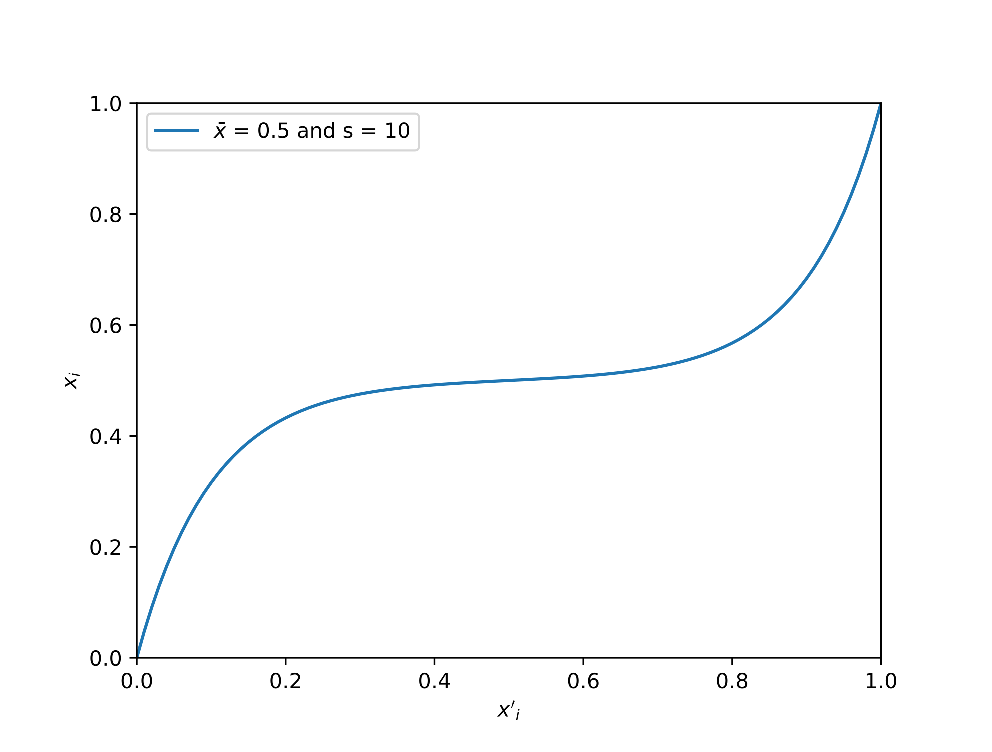
\includegraphics[scale=.5]{Images/MVMOTransformation.eps}
	\end{center}
	\label{fig: mappingf}
\end{figure}

\begin{figure}[h]
	\caption{Effect of different mean and shape factor values on mapping function}
	\begin{center}
		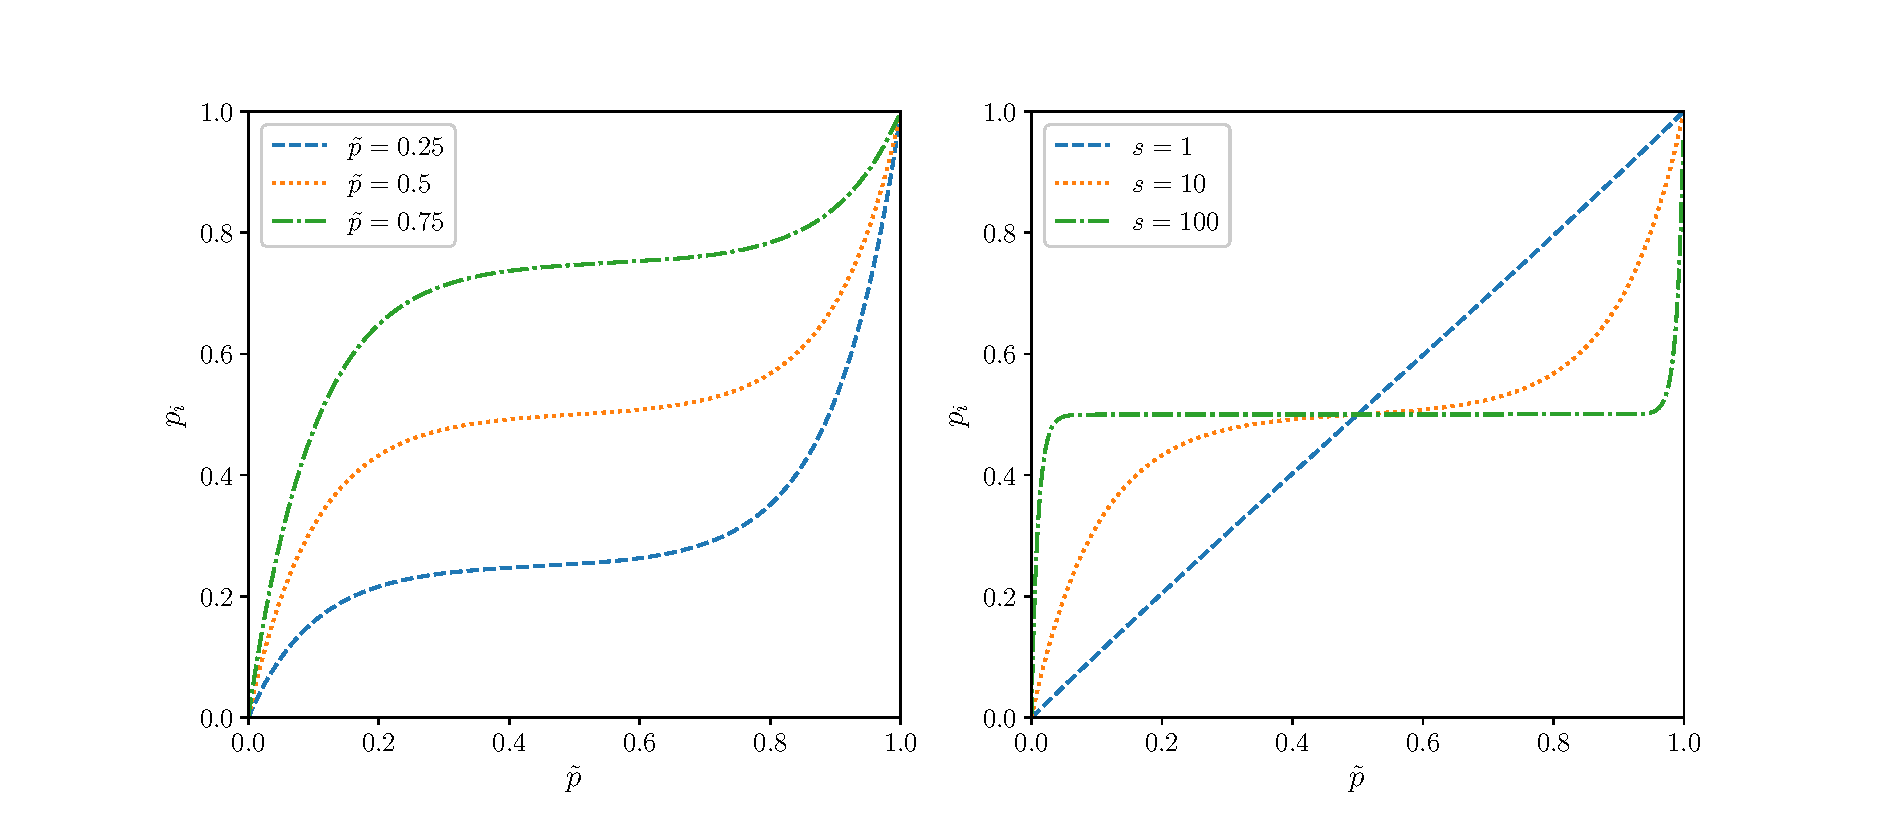
\includegraphics[scale=.5]{Images/mean_var_effects.eps}
	\end{center}
	\label{fig: mapeffects}
\end{figure}

As shown in \eqref{eq: hfunc}, two shape factors are used to evaluate the function. Different values of shape factors emphasizes the search below or above mean value. Thus, by controlling the values $s_{i1}$ and $s_{i2}$, the method can prioritize exploration (global search) or exploitation (local search) on a given region. Figure \ref{fig: diffs} depicts how asymmetrical shape factors affect the mapping function.

\begin{figure}[h]
	\caption{Comparison between symmetrical and asymmetrical shape factors}
	\begin{center}
		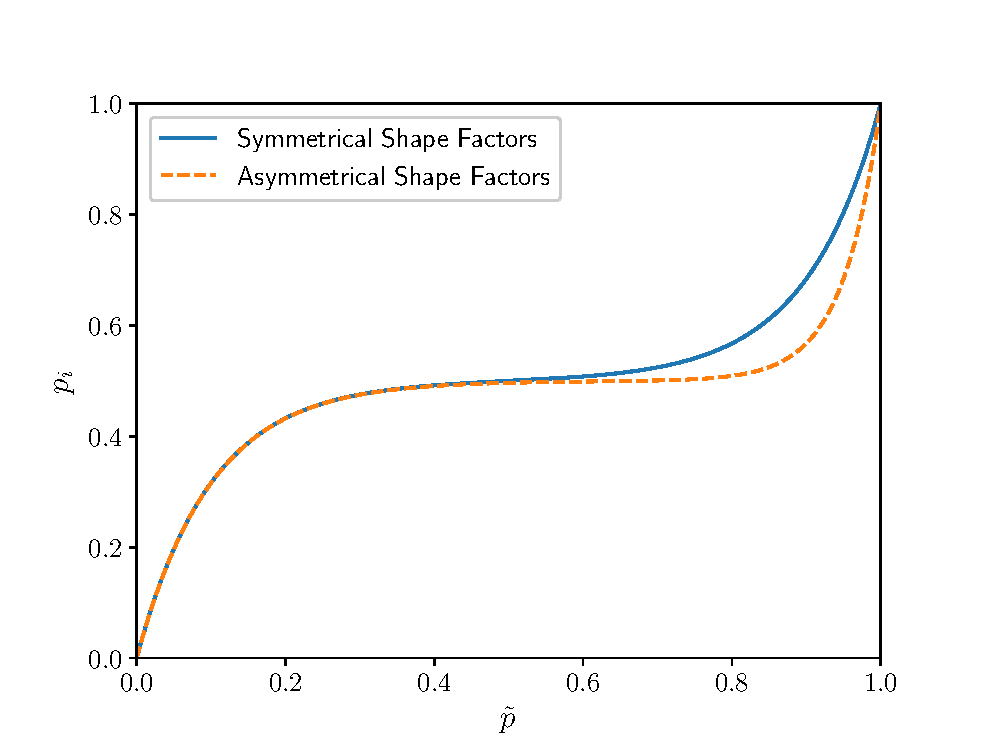
\includegraphics[scale=.5]{Images/symmetrical_transf.eps}
	\end{center}
	\label{fig: diffs}
\end{figure}

The final step during offspring generation is crossover. During this phase, the mutated genes are united with the remaining genes inherited from parent, forming the new individual. This new individual is evaluated and included to the population if it is better than, at least, the population's worst individual. This process goes on until at least one stop criterion has been fulfilled.

The main advantages of this method are low computational cost, good performance using small populations, constrained search region, preventing divergence, and the fact that it is non-specific. On the other hand, this method, as other metaheuristics, takes a great amount of time to converge when its error approaches zero.

\section{Trajectory Sensitivity Method}

Considering a nonlinear system described by \eqref{eq: xdot}, in order to minimize the error between model and real system, given by \eqref{eq: J(p)}, one must discover a parameter vector $p^{*}$ such as:

\begin{equation}
	G(p^{*}) = \frac{\partial J(p^{*})}{\partial p} = 0
\end{equation}

This derivative can be written as:

\begin{equation}	
	G(p) = -\int\displaylimits_{0}^{T_{0}} \left(\frac{dy}{dp}\right)^{T} (y_{r} - y) dt
	\label{eq: G(p)}
\end{equation}

Truncating the Taylor series for $G(p)$ on the first-order term results on \eqref{eq: Taylor}. The matrix $\Gamma$ is described in \eqref{eq: Gamma}.

\begin{equation}
	G(p^{*}) = G(p) + \Gamma (p)(p^{*} - p)
	\label{eq: Taylor}
\end{equation}

\begin{equation}
	\Gamma (p) = \frac{\partial G(p)}{\partial p} \approx \int\displaylimits_{0}^{T_{0}} \left(\frac{dy}{dp}\right)^{T} \left(\frac{dy}{dp}\right) dt
	\label{eq: Gamma}
\end{equation}

By rearranging the terms on \eqref{eq: Taylor}, the following equation is obtained. It describes how the parameters are updated after the $n^{th}$ iteration.

\begin{equation}
	p^{n+1} = p^{n} + \Gamma^{-1}(p^{n})\cdot G(p^{n})
\end{equation}

Obtaining the Jacobian matrix (also called trajectory sensitivity matrix) $\frac{\partial y}{\partial p}$, used in \eqref{eq: G(p)} and \eqref{eq: Gamma}, analytically is a hard task. However, by applying the definition of derivative, given by \eqref{eq: deriv}, the sensibilities can be approximated without any analytical derivation of the equations.

\begin{equation}
	\frac{df(x)}{dx} = \lim\limits_{\delta \to 0} \frac{f(x + \delta) - f(x)}{\delta}
	\label{eq: deriv}
\end{equation}

Consider two parameter vectors $p$ and $p^{\epsilon}$, where $p^{\epsilon}$ is obtained by adding a small perturbation $\epsilon p_{i}$ to the $i-th$ element of $p$, as shown in \eqref{eq: pvecs}.

\begin{equation}
	p = 
	\begin{bmatrix}
		p_{1} \\
		\vdots \\
		p_{i} \\
		\vdots \\
		p_{n}
	\end{bmatrix}; \ \ \ \ 
	 p^{\epsilon} =
	\begin{bmatrix}
		p_{1} \\
		\vdots \\
		p_{i} + \epsilon p_{i} \\
		\vdots \\
		p_{n}
	\end{bmatrix}
	\label{eq: pvecs}
\end{equation}

With $\epsilon$ sufficiently small, the partial derivative with respect to the parameter $p_{i}$ can be approximated by the difference shown in equation \eqref{eq: diff}. The value of $\epsilon = 0.1 \times 10^{-3}$ have shown great results for most cases. Using the approximation of the partial derivatives allows Trajectory Sensitivity method to be applied on both differentiable and non-differentiable systems \cite{Benchluch1993}, \cite{Cari2006}.

\begin{equation}
	\frac{\partial y(x, p, u)}{\partial p_{i}} \approx \frac{y(x, p^{\epsilon}, u) - y(x, p, u)}{\epsilon p_{i}}
	\label{eq: diff}
\end{equation}

The Trajectory Sensitivity Method has fast convergence characteristics and can applied directly to nonlinear problems, not requiring linearization. Also, by analyzing the sensitivities, the method provides information about identifiability of parameters. However, TSM is very sensitive to initial value of parameter chosen as starting point. Thus, if the initial values are too far from the real values, the method can either diverge or converge to wrong values. Besides, the information provided to the method must contain the effects of the parameters, otherwise they won't be observable \cite{Benchluch1993}.

\section{Hybrid Estimation Method}
\label{sec: Hybrid_Method}

By associating MVMO and TSM, the hybrid estimation approach applied in this work combines most benefits of both methods whilst mitigating their disadvantages. The resulting method has smaller convergence time when compared to MVMO alone and is less sensitive to initial values of parameters than TSM. The flowchart depicted in Figure \ref{fig: flowchart} illustrates how this method works.

\begin{figure}[h]
	\caption{Flowchart of hybrid estimation method}
	\begin{center}
		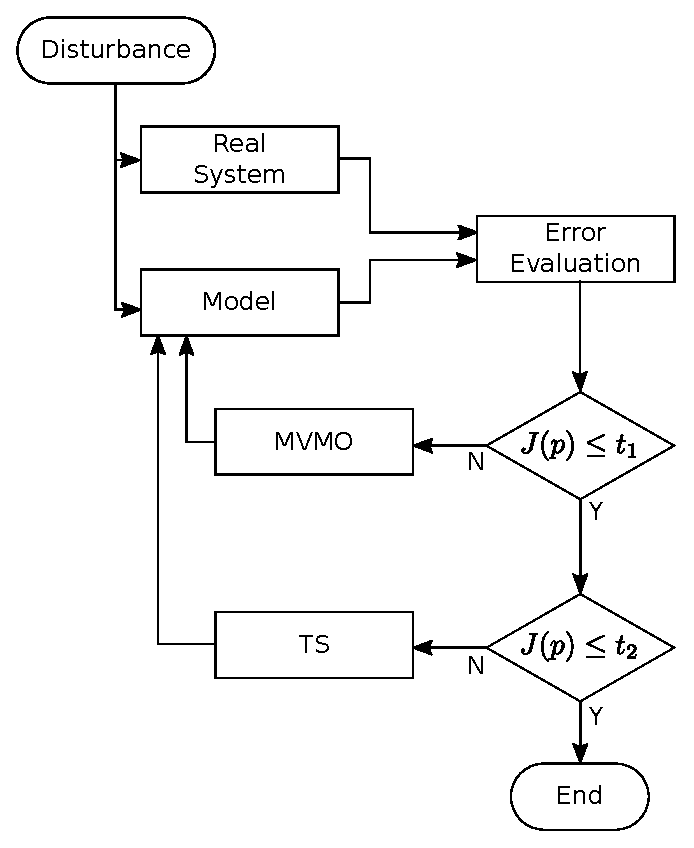
\includegraphics[scale=0.7]{Images/Flowchart.eps}
	\end{center}
	\label{fig: flowchart}
\end{figure}

At first, a set of measurement data are recorded in the "Real System" block. These measurement must contain information of the dynamic response of the system. After that, some measurement are used as input to the block "Model", which is composed of equations of the mathematical model. The output of the "Real System" and "Model" are compared to evaluate the error function $J(p)$. While $J(p)$ is greater than a given tolerance $tol_{1}$, MVMO algorithm will look for possible optimal solutions across the search region. Afterwards, the error will eventually drop to a value lower than $tol_{1}$, and TSM will be used to refine the search to an optimal solution, with error level below tolerance $tol_{2}$.

In order to assess the parameter estimation methods (TSM, MVMO and hybrid method), the parameter estimation of spring-mass model was conducted and its results are shown in the following section. The spring-mass is a nonlinear dynamic system and was chosen for this assessment due to its simplicity and reduced order.

\section{Parameter Estimation of Spring-Mass Model}

The spring-mass system is a simple mathematical model often used as example of dynamic systems. It is composed of an object of mass $m$ connected to a fixed point in space by a spring of stiffness constant $k$. The mass is on a surface with no friction and oscillates when disturbed by an external force $\vec{F}$. The system is depicted in Figure \ref{fig: spring_mass}.

\begin{figure}[h]
	\caption{Spring-mass system}
	\begin{center}
		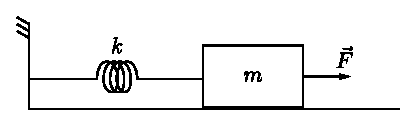
\includegraphics[scale=1]{Images/spring_mass.eps}
	\end{center}
	\label{fig: spring_mass}
\end{figure}

By applying Newton's laws of motion on the system shown above, one can easily deduct that the movement of the mass is described by \eqref{eq: SpringMass}. The mass position is represented by $x$, while $v$ and $a$ correspond to its speed and acceleration, respectively.

\begin{equation}
	\begin{cases}
		\dot{v} = x \\
		\dot{a} = \frac{k}{m}v - \frac{F}{m}
	\end{cases}
	\label{eq: SpringMass}
\end{equation}

This system can be interpreted as of \eqref{eq: xdot}, with the state, input, output and parameter vectors given by \eqref{eq: spring_mass_x}, \eqref{eq: spring_mass_u}, \eqref{eq: spring_mass_y} and \eqref{eq: spring_mass_p}, respectively.

\begin{equation}
	x = [v, a]^{T}
	\label{eq: spring_mass_x}
\end{equation}

\begin{equation}
	u = [F]
	\label{eq: spring_mass_u}
\end{equation}

\begin{equation}
	y = [v, a]^{T}
	\label{eq: spring_mass_y}
\end{equation}

\begin{equation}
	p = [m, k]^{T}
	\label{eq: spring_mass_p}
\end{equation}

The initial values of $v$ and $a$ are needed in order to solve the ordinary differential equation given by \eqref{eq: SpringMass}. Those values, as well as the magnitude of $\vec{F}$\ are given by:

\begin{equation}
	\begin{cases}
		v(t=0) = 0\ m/s\\
		a(t=0) = 0\ m/s^{2}
	\end{cases}
\end{equation}

\begin{equation}
	F(t\geq 0) = 4\ N
\end{equation}

The system was simulated with parameters set at $m = 3\ kg$ and $k = 6\ N/m$ and the output behaviour obtained was used as reference for the estimation. Three different estimation processes were executed: TSM, MVMO and the hybrid approach of MVMO and TSM combined. The tolerance for all three estimations was set at $tol = 0.1$.

\subsection{Trajectory Sensitivity Estimation}

It took 7 iterations (10 seconds on a PC) for Trajectory Sensitivity Method to estimate the parameters when the initial values were $m_{0} = 7\ kg$ and $k_{0} = 7\ N/m$. The final error of the estimation process was $1.90\times 10^{-3}$. This shows how fast and precise this method is, as long as the initial values chosen are in the neighbourhood of the real parameters. Figure \ref{fig: TS_conv} shows the error evolution during estimation suing TSM while Table \ref{tab: spring_mass_ts} displays the values estimated for each parameter.

\begin{figure}[h]
	\caption{Error evolution of TSM with $m_{0} = 7\ kg$ and $k_{0} = 7\ N/m$}
	\begin{center}
		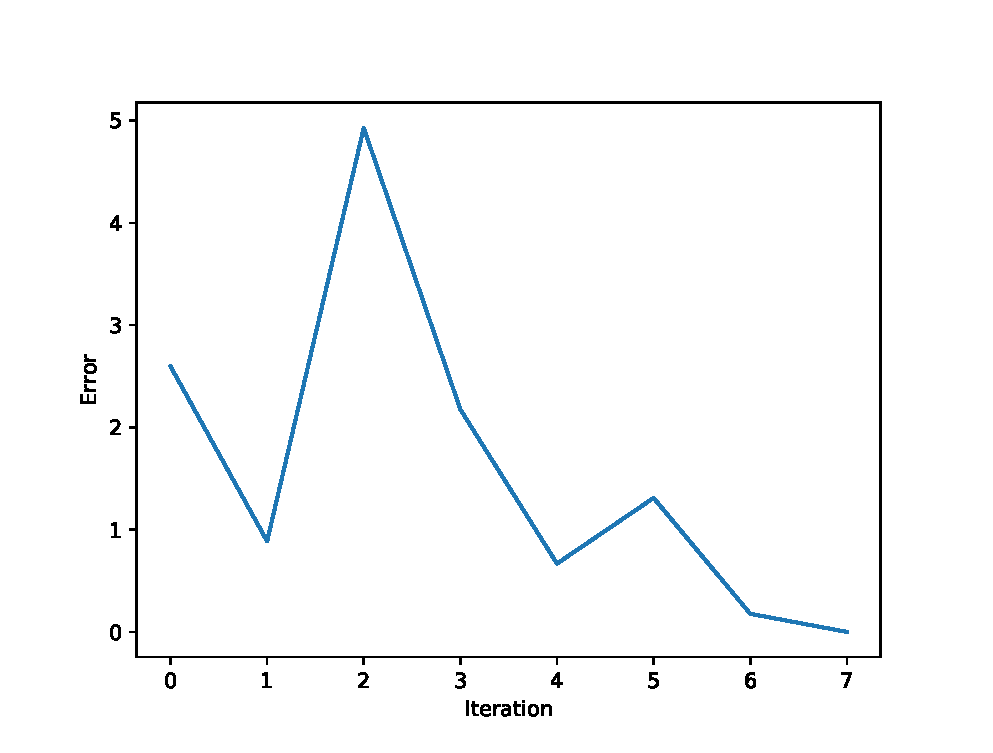
\includegraphics[scale=0.6]{Images/spring_mass_ts_conv.eps}
	\end{center}
	\label{fig: TS_conv}
\end{figure}

\begin{table}[h]
	\caption{Parameters estimated by Trajectory Sensitivity Method}
	\begin{center}
		\begin{tabular}{c|c|c}
			Parameter & \shortstack{Estimated \\ value} & \shortstack{Real \\ value} \\
			\hline
			$m$ & 3.080 & 3 \\
			$k$ & 6.145 & 6 \\
		\end{tabular}
	\end{center}
	\label{tab: spring_mass_ts}
\end{table}

However, the convergence region \footnote{Convergence region is a region in parameter space where, if the initial guess for parameter values is inside it, the convergence to true values is guaranteed.} of TSM is limited, diverging for initial points far enough from the real values. The convergence region for the real values was obtained in \cite{Ecyo} and is shown in Figure \ref{fig: conv_reg}. For comparison, the MVMO and the hybrid approach converge for the entire search region displayed on the graph.

\begin{figure}[h]
	\caption{Convergence region of Trajectory Sensitivity Method}
	\begin{center}
		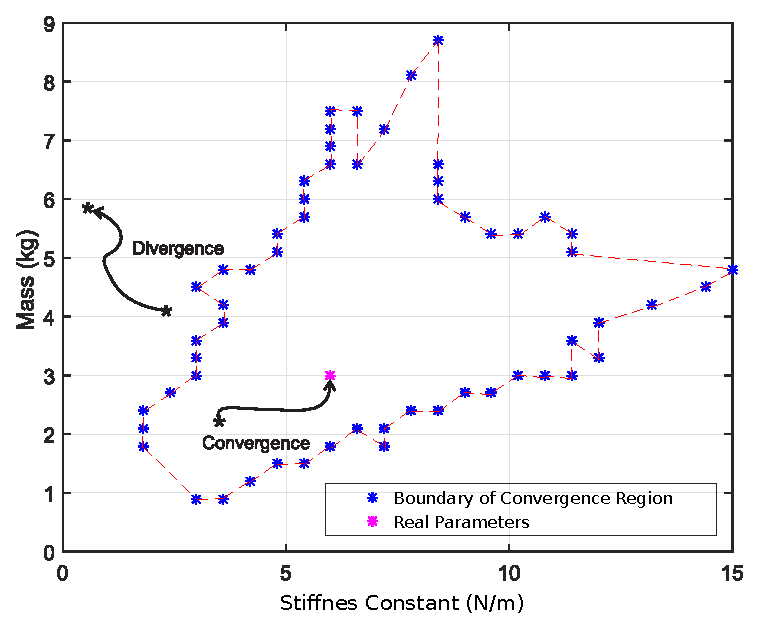
\includegraphics[scale=0.6]{Images/Conv_reg.eps}
	\end{center}
	\label{fig: conv_reg}
	\legend{Source: Adapted from \cite{Ecyo}}
\end{figure}

To illustrate the importance of good initial values, the parameters were reestimated using TSM, but now it was selected initial values $m_{0} = 8\ kg$ and $k_{0} = 10\ N/m$ outside the convergence region. Notice that these values are not too far from the ones used in the previous estimation. The results, on the other hand, were extremely different. The method was not able to lower $J(p)$ below $16.4$ and the parameters converged to different values $m_{f} = 2.7\ kg$ and $k_{f} = 118.6\ N/m$. The error evolution for this estimation is depict in Figure \ref{fig: TS_nconv}.

\begin{figure}[h]
	\caption{Error evolution of TSM with $m_{0} = 8\ kg$ and $k_{0} = 10\ N/m$}
	\begin{center}
		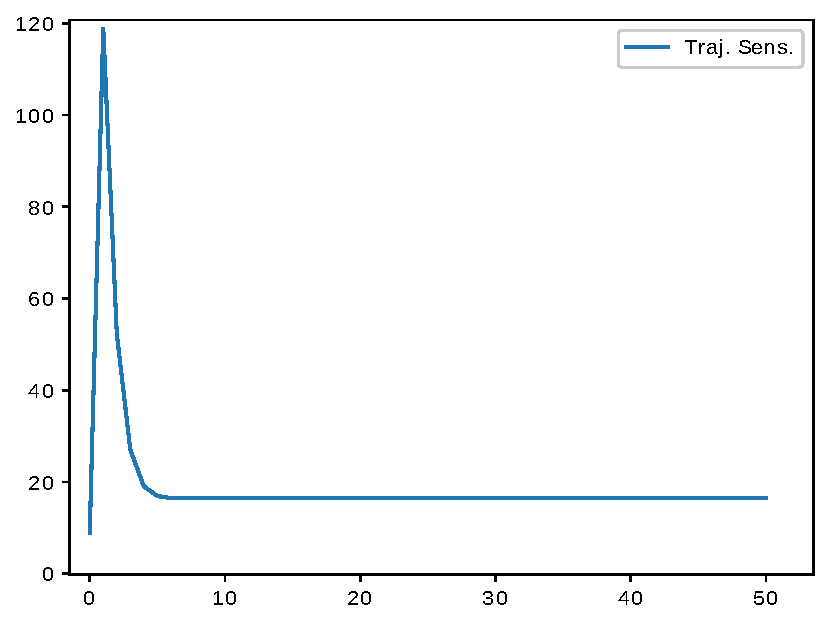
\includegraphics[scale=0.6]{Images/TS_nconv.eps}
	\end{center}
	\label{fig: TS_nconv}
\end{figure}

\subsection{MVMO Estimation}

In order to estimate the parameter using MVMO, a search region in parameter space must be defined first. By the fact that MVMO will be compared to TSM, the parameter boundaries obtained from TSM convergence region displayed in Figure \ref{fig: conv_reg}. The limits chosen define a region where TSM convergence is almost always guaranteed for any starting point inside of it. Figure \ref{fig: spring_mass_MVMO_region} displays the search region chosen for MVMO estimation and Table \ref{tab: spring_mass_MVMO_bounds} presents the parameter boundaries selected.

\begin{figure}[h]
	\caption{Search region chosen for MVMO}
	\begin{center}
		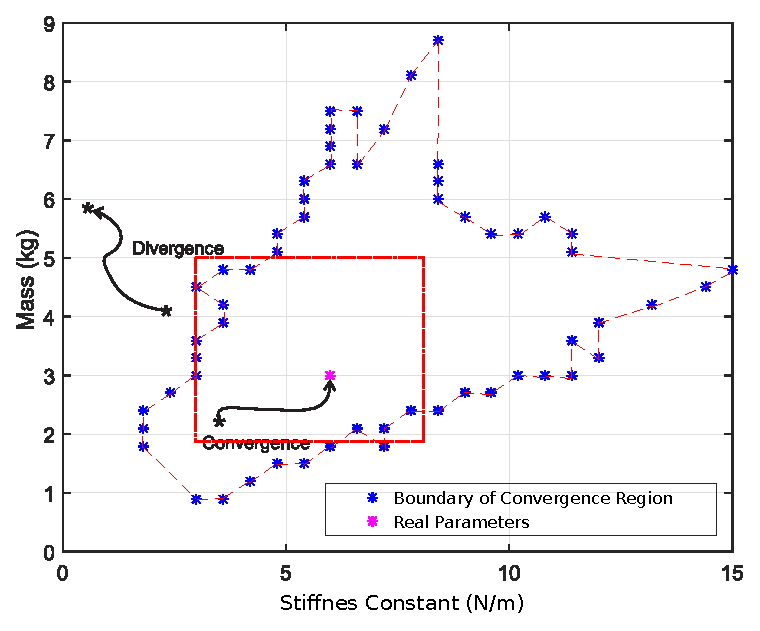
\includegraphics[scale=0.6]{Images/search_region_MVMO.eps}
	\end{center}
	\label{fig: spring_mass_MVMO_region}
\end{figure}

\begin{table}[!h]
	\centering
	\caption{MVMO parameter boundaries}
	\begin{tabular}{c|cc}
		Parameter & \shortstack{Lower \\ boundary} & \shortstack{Upper \\ boundary} \\\hline
		$m$ & 1.9 & 5 \\
		$k$ & 3 & 8 \\
	\end{tabular}
	\label{tab: spring_mass_MVMO_bounds}
\end{table}

The effects of population size were evaluated by running estimations for 4 different values: 5, 10, 20 and 50 individuals. For each population size, 35 estimation process were conducted with tolerance of $tol = 0.1$, maximum number of generation equals to $n_{gen}=1000$ and one new individual generated at each generation. The average number of generations, duration and estimated parameter values ($\bar{m}$ and $\bar{k}$) for each population size evaluated is shown in Table \ref{tab: spring_mass_MVMO_size}.

\begin{table}[!h]
	\centering
	\caption{MVMO parameter boundaries}
	\begin{tabular}{c|cccc}
		\shortstack{Population \\ size} & \shortstack{Average \\ \# of generations} & \shortstack{Average \\ duration (s)} & $\bar{m}$ & $\bar{k}$ \\
		\hline
		5 & 71 & 32.23 & 3.23 & 6.20 \\
		10 & 27 & 15.43 & 3.38 & 6.05 \\
		20 & 5 & 10.22 & 3.45 & 5.96 \\
		50 & 1 & 20.72 & 3.66 & 5.76 \\
	\end{tabular}
	\label{tab: spring_mass_MVMO_size}
\end{table}

From these results, one can infer that the optimal population size for estimating the parameter of the spring-mass model is around 20 individuals. It can also be noticed that, despite converging on the first generation, populations of size 50 usually take more time to than others due to the large amount of individuals that must be generated and evaluated at the start of the estimation.

Figure \ref{fig: MVMO_conv} depicts the error evolution for one of the 35 estimations conducted for a population of 20 individuals. The heuristic method converged after 21 generations, with estimated values of $m=2.6\ kg$ and $k=5.2\ N/m$.

\begin{figure}[h]
	\caption{Error evolution of MVMO}
	\begin{center}
		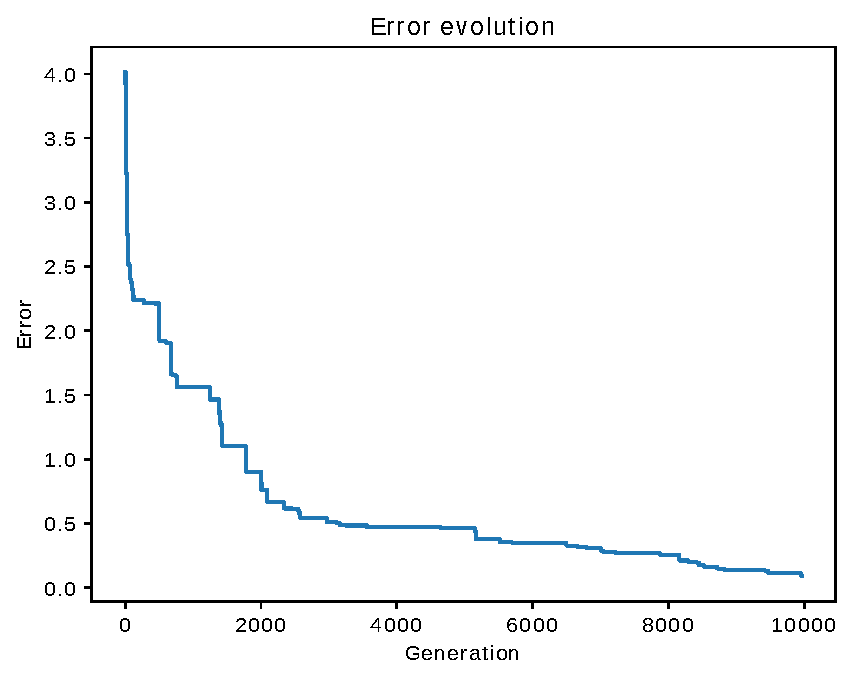
\includegraphics[scale=0.6]{Images/MVMO_conv.eps}
	\end{center}
	\label{fig: MVMO_conv}
\end{figure}

\subsection{Hybrid Estimation}

By combining both methods, the hybrid approach benefits from the quick error reduction provided by MVMO and the fast convergence from TSM when inside convergence region. The tolerance for this approach were set at $tol_{1} = 0.5$ (MVMO) and $tol_{2} = 0.1$ (TSM). The population size was set at 20 individuals according to the results obtained in the previous section. Parameters of the spring-mass system were estimated using this method for 35 times and the average estimation time was $11.65\ s$.

Figure \ref{fig: Hybrid_conv} depicts the error evolution for one of the 35 estimations conducted. The hybrid estimation method converged after 3 iterarions, with estimated values of $m=3.063\ kg$ and $k=6.134\ N/m$.

\begin{figure}[h]
	\caption{Error evolution with of hybrid approach for spring-mass system}
	\begin{center}
		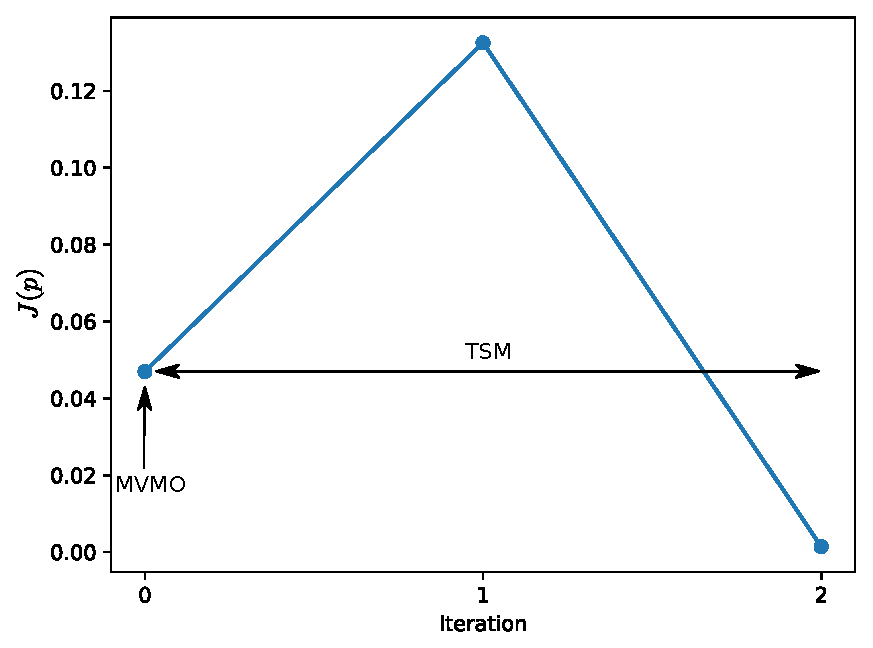
\includegraphics[scale=0.7]{Images/Hybrid_conv_.eps}
	\end{center}
	\label{fig: Hybrid_conv}
\end{figure}

When compared to each method, the hybrid approach converges faster than MVMO but slower than TSM, as shown in Table \ref{tab: SM}. Although all methods converged to parameter values that resulted in an error level below the tolerance, TSM and the Hybrid approach provided final results with error level below the values obtained by MVMO.

\begin{table}[h]
	\caption{Comparison of approaches}
	\begin{center}
	\begin{tabular}{c|c|c|c|c|c}
		Approach & Tolerance & $\bar{m}$ &$\bar{k}$ & \shortstack{Processing \\ Time (s)} & \shortstack{Final Error \\ $J(p)$} \\
		\hline
		TSM  & 0.1 & 3.08 & 6.15 & $7 \ s$  & $2.76\times 10^{-3}$ \\
		\hline
		MVMO  & 0.1 & 3.45 & 5.96 & $10\ s$  & $52.32\times 10^{-3}$\\
		\hline
		Hybrid  & \shortstack{$tol_{1}=0.5$ \\ $tol_{1}=0.1$} & 3.08 & 6.15 & $12\ s$  & $24.46\times 10^{-3}$
	\end{tabular}
	\end{center}
	\label{tab: SM}
\end{table}

The great advantage of the hybrid method is the increment of success in the convergence of parameters to the true value. This way, the MVMO approach is only used as an "inteligent initial guess".
